\chapter{Systemarkitektur}

Dette afsnit præsenterer systemets arkitektur i en grad der gør det muligt at forstå sammensætningen mellem dets hardware og software komponenter.

\section{Domænemodel}

På figur \ref{figure:domainModel} ses domænemodellen af systemet. Denne har til formål at præsentere forbindelserne mellem systemets komponenter, samt dets grænseflader.

\begin{figure}[H]
	\centering
	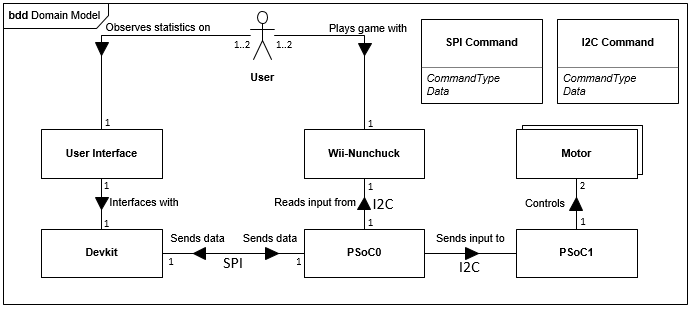
\includegraphics[width=\textwidth]{SystemArkitektur/images/DomainModel.PNG}
	\caption{Systemets domænemodel}
	\label{figure:domainModel}
\end{figure}

Her repræsenteres hardware som blokke forbundet med associeringer. Associeringerne viser grænsefladerne mellem de forbundne hardware komponenter (Enten \textit{SPI} eller \textit{I2C}), samt retningen af kommunikationen. Af modellen fremstår konceptuelle kommandoer for grænsefladerne, som beskriver deres nødvændige attributter.

\section{Software Allokering}

Domænemodellen i figur \ref{figure:allocationDiagram} præsenterer systemets hardwareblokke. På figur \ref{figure:allocationDiagram} ses et software allokeringsdiagram, som viser hvilke hardwareblokke der har softwaredele af systemet allokeret på sig. 

\begin{figure}[H]
	\centering
	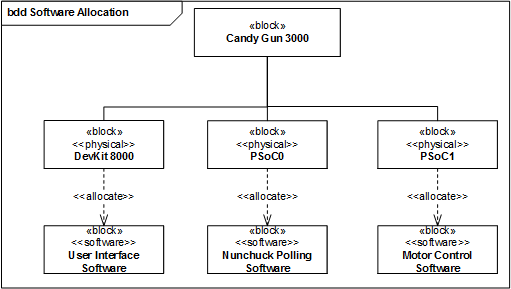
\includegraphics[width=\textwidth]{SystemArkitektur/images/SoftwareAllocation.PNG}
	\caption{Systemets software allokeringer}
	\label{figure:allocationDiagram}
\end{figure}

Det kan her ses at systemet består af tre primære softwaredele: \textit{DevKit 8000 Software}, \textit{PSoC0 Software}, \textit{PSoC1 Software}. Disse er fordelt over de 3 tilsvarende CPU'er. Der henvises til til \textbf{APPLIKATIONSMODELLER} for overblik over de konceptuelle klasser der indgår i disse softwaredele. Her gives blot en forståelse for hvor systemets software hører til.

\section{Hardware}

\subsection{BDD}

På figur \ref{figure:bddDiagram} ses BDD'et for systemet.

\begin{figure}[H]
	\centering
	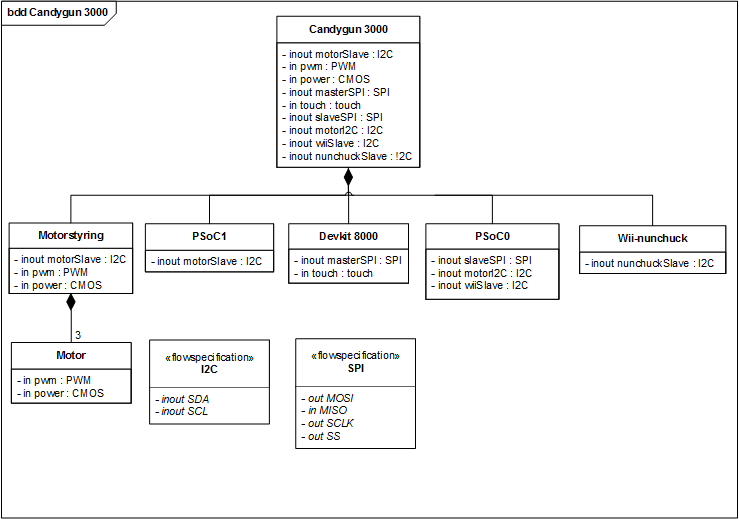
\includegraphics[width=\textwidth]{SystemArkitektur/images/BDD_overordnet.PNG}
	\caption{BDD af systemets hardware}
	\label{figure:bddDiagram}
\end{figure}

Her vises alle hardwareblokke fra domænemodellen (figur \ref{figure:domainModel}) med nødvændige indgange og udgange for de fysiske signaler. Yderligere ses det at flow specifikationer er defineret for de ikke-atomare forbindelser \textit{I2C} samt \textit{SPI}, da disse er busser bestående af flere forbindelser. Der henvises til \textbf{IBD AFSNIT} for en detaljeret model af de fysiske forbindelser mellem hardwareblokkende.

\subsection{IBD}

På figur \ref{figure:ibdDiagram} ses IBD'et for systemet.

\begin{figure}[H]
	\centering
	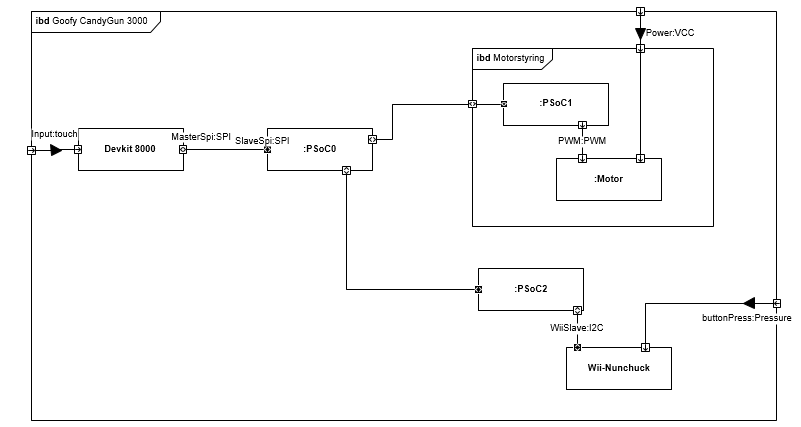
\includegraphics[width=\textwidth]{SystemArkitektur/images/GoofyCandyIBDImageRev2.PNG}
	\caption{IBD af systemets hardware}
	\label{figure:ibdDiagram}
\end{figure}

Her vises alle hardwareblokke med de fysiske forbindelser beskrevet i BDD'et (figur \ref{figure:bddDiagram}). 

Det ses at systemet bliver påvirket af tre eksterne signaler: \textit{touch}, \textit{input}, samt \textit{voltage}. \textit{touch} er input fra brugeren når der interageres med brugergrænsefladen. \textit{input} er brugerens interaktion med Wii-Nunchuk. \textit{voltage} er forsyningsspænding til systemet.

\section{Software}

\subsection{SPI Kommunikations Protokol}

\subsection{I2C Kommunikations Protokol}

I afsnittet \textbf{IBD} ses det på IBD'et (figur \ref{figure:ibdDiagram}) at tre hardwareblokke kommunikerer med hinanden via en I2C bus. Til denne I2C kommunikation er der defineret en protokol, som sætter en standard for hvordan modtaget data skal fortolkes. Denne protokol beskrives her.

I2C gør brug af en indbygget protokol der anvender adressering af hardware-enheder for at identificere hvilken enhed der kommunikeres med. Derfor har hardwareblokkene som indgår i I2C kommunikation fået tildelt adresser. På tabel \ref{table:I2CAddress} ses adresserne tildelt systemets PSoCs.

\begin{table}[H]
	\centering
	\begin{tabular}{llllllllll}
		\hline
		\multicolumn{1}{|l|}{I2C Adresse bits} & 7                        & 6                        & 5                        & 4 & 3 & 2 & \multicolumn{1}{l|}{1} & \multicolumn{1}{l|}{0 (R/W)} \\ \hline
		\rowcolor[HTML]{CBCEFB} 
		{\color[HTML]{000000} PSoC0}           & {\color[HTML]{000000} 0} & {\color[HTML]{000000} 0} & {\color[HTML]{000000} 0} & 1 & 0 & 0 & 0                      & 0/1                          \\
		PSoC1                                  & 0                        & 0                        & 0                        & 1 & 0 & 0 & 1                      & 0/1 \\
		\rowcolor[HTML]{CBCEFB} 
		{\color[HTML]{000000} Wii-Nunchuck}           & {\color[HTML]{000000} 1} & {\color[HTML]{000000} 0} & {\color[HTML]{000000} 1} & 0 & 0 & 1 & 0                      & 0/1                      
	\end{tabular}
	\caption{Adresser der anvendes på I2C bussen}
	\label{table:I2CAddress}
\end{table}

Da I2C dataudveksling sker bytevist, er kommunikations protokollen opbygget ved, at kommandoens type indikeres af den første modtagne byte. Herefter følger \textit{N}-antal bytes som er kommandoens tilhørende data. \textit{N} er et vilkårligt heltal og bruges i dette afsnit når der refereres til en mængde data-bytes der sendes med en kommandotype.

Kommandoens type definerer antallet af databytes modtageren skal forvente og hvordan disse skal fortolkes. På figur \ref{fig:I2CProtokolEksempel} ses et sekvensdiagram der, med pseudo-kommandoer, demonstrerer forløbet mellem en I2C afsender og modtager ved brug af kommunikations protokollen.

\begin{figure}[H]
	\centering
	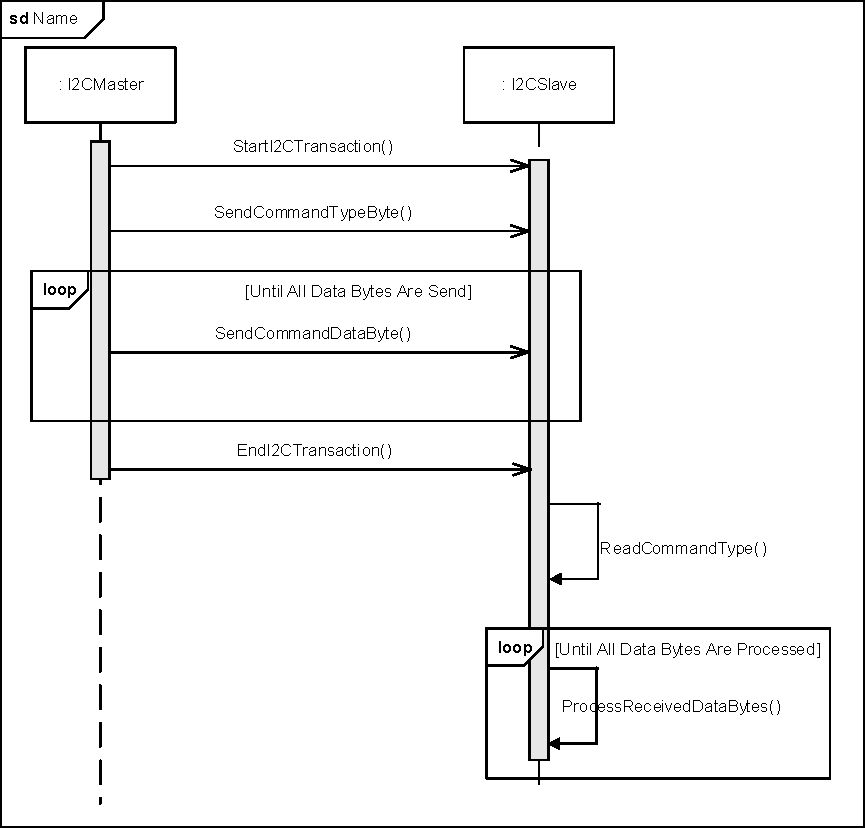
\includegraphics[width=\textwidth] {Systemarkitektur/images/I2CProtocol}
	\caption{Eksempel af I2C Protokol Forløb}
	\label{fig:I2CProtokolEksempel}
\end{figure}

På figur \ref{fig:I2CProtokolEksempel} ses at afsenderen først starter en I2C transaktion, hvorefter typen af kommando sendes som den første byte. Efterfølgende sendes \textit{N} antal bytes, afhængig af hvor meget data den givne kommandotype har brug for at sende. Efter afsluttet I2C transaktion læser I2C modtageren typen af kommando, hvor den herefter kan fortolke \textit{N} antal modtagne bytes afhængig af den modtagne kommandotype.

På tabel \ref{table:I2CKommandoer} ses de definerede kommandotyper og det tilsvarende antal af bytes der sendes ved dataveksling.

\begin{table}[H]
	\centering
	\resizebox{\textwidth}{!}{
		\begin{tabular}{lllll}
			\hline
			\multicolumn{1}{|l|}{Kommandotype}    & \multicolumn{1}{l|}{Beskrivelse}                                            & \multicolumn{1}{l|}{Binær Værdi} & \multicolumn{1}{l|}{Hex Værdi} & \multicolumn{1}{l|}{Data Bytes}                                                                                         \\ \hline
			\rowcolor[HTML]{CBCEFB} 
			{\color[HTML]{000000} NunchchuckData} & {\color[HTML]{000000} Indeholder aflæst data fra Wii Nunchuck controlleren} & 0010 1010                        & 0xA2                           & \begin{tabular}[c]{@{}l@{}}Byte \#1 Analog X-værdi\\ Byte \#2 Analog Y-værdi\\ Byte \#3 Analog Buttonstate\end{tabular} \\
			I2CTestRequest                        & Anmoder PSoC0 om at starte I2C-kommunikations test                          & 0010 1001                        & 0x29                           & Ingen databyte                                                                                                          \\
			\rowcolor[HTML]{CBCEFB} 
			I2CTestAck                            & Anmodning om at få en I2C OK besked fra I2C enhed                           & 0010 1000                        & 0x28                           & Ingen databyte                                                                                                         
		\end{tabular}
	}
	\caption{Kommandotyper der anvendes ved I2C kommunikation}
	\label{table:I2CKommandoer}
\end{table}

Kolonnerne "Binær Værdi" og "Hex Værdi" i tabel \ref{table:I2CKommandoer} viser kommandotypens unikke tal-ID i både binær- og hexadecimalform. Denne værdi sendes som den første byte, for at identificere kommandotypen. 

\section{Signalbeskrivelse}
	\begin{tabular}{|>{\hspace{0pt}}p{1.5cm}  >{\hspace{0pt}}p{3cm} | p{2.5cm} | p{2.5cm} | p{2.5cm} |}
		\hline
		\textbf{Blok-navn} & \textbf{Funktionsbeskrivelse} & \textbf{Signaler} & \textbf{Kommentar} & 3\\ \hline
		Mål & & Klarhed om projekt idé, samt de vigtigste krav bla bla bla bla & blabla & blabla\\ \hline
		Længde & & 1 uge & 3 uger & 3 uger\\ \hline
		Disciplin & Artefakt & Inception 1 & ... & ...\\ \hline
		\textbf{Projekt Formulering} & hey hey hey hey & Udled projektformulering. Anvend MosCoW til at bla bla bla & & \\ \hline
		\textbf{\hspace{0pt}Specifikation} & Kravspecifikation \& Accepttest & ... & ... & ... \\ \hline
		\textbf{Arkitektur} & Systemarkitektur & Ingen & bla bla & bla bla \\ \hline
		\textbf{Design} & Design dokumentation & Ingen & bla bla & bla bla\\ \hline
		\textbf{Implementering og modul test} & HW/SW/Mekanik & Ingen & bla bla & bla bla \\ \hline
		\textbf{Projekt styring} & Projekt plan & bla bla & bla bla & bla bla \\ \hline
		\end{tabular}
\subsection{Specifikation og Analyse}